\documentclass[11pt,a4paper]{article}

\usepackage[a4paper,margin=0.8in]{geometry}
\usepackage{xeCJK}
\usepackage{booktabs}
\usepackage{amsmath,amssymb}
\usepackage{array}
\usepackage{graphicx}
\usepackage{caption}
\usepackage{enumitem}
\usepackage{float}
\usepackage{algorithm}
\usepackage{algorithmicx}
\usepackage{algpseudocode}
\usepackage{setspace}
\usepackage[colorlinks=true, linkcolor=blue, urlcolor=blue, citecolor=blue]{hyperref}

% 調整行距以符合長篇報告閱讀舒適度
\setstretch{1.15}

\title{\textbf{Algorithmic Roster Construction: \\ Strategic Talent Acquisition under Competitive Scarcity} \\[0.5em]
\large A Fantasy Baseball Testbed for Optimization and Real-Time Heuristics\thanks{Source code and data: \url{https://github.com/089487/OR_Final_Project}} \\[1em]
\normalsize OR114-2 Final Project, Group 4}
\author{
B13705051 周孟承 \and
B13902103 鄭宇宏 \and
B13303153 詹舒宇 \and
B11705039 李盈盈
}
\date{}

\begin{document}
\maketitle

\vspace{-3em}  % 這裡的數字可以調整，-3em 左右通常能顯著縮減間距


% \begin{abstract}
% In this report, we study a \textbf{sequential resource allocation problem under competitive scarcity}. We utilize \textbf{Fantasy Baseball as a data-rich testbed} due to its complex roster constraints and high-frequency market dynamics. For modern sports organizations, identifying talent is only one part of the challenge; the true competitive edge lies in the \textbf{strategy of draft execution}. While traditional Integer Programming (IP) provides a mathematical benchmark, it fails to scale to massive player pools under real-time pressure. We propose the \emph{Opportunity Cost Greedy (OCG)} algorithm, which captures the \textbf{cost-of-delay} by forecasting future asset availability. Our results across synthetic and real-world 2026 data show that OCG achieves near-optimal performance in seconds, effectively functioning as a scalable decision-support framework.
%  \end{abstract}

\section{Introduction: The General Manager's Dilemma}

As the 2026 MLB season approaches, front offices across the league are focused on one critical objective: the championship. The cornerstone of a winning season is not just how the players perform on the field, but how they are selected during the off-season draft. Developing a "winning strategy" to build an elite team is the primary concern of professional General Managers and the obsession of millions of fans participating in online simulations such as Fantasy Baseball. Regardless of the platform, the core problem remains the same: how does a manager use a limited sequence of picks to secure the highest possible utility before opponents deplete the talent pool?

The draft represents a critical portfolio optimization puzzle for modern sports roster construction. In an era where scouting analytics and player evaluations have largely converged, the competitive edge has shifted from merely identifying talent to the strategy of execution. This project models the draft process as a sequential resource acquisition problem, using Fantasy Baseball as a high-fidelity competitive testbed to study how decision-makers can maximize objective value under strict structural constraints and intense market competition.

The motivation for this study stems from the inherent complexity of a draft environment, which forces managers to confront a fundamental "Timing Paradox" — the challenge of securing a specific asset now before market timing and positional scarcity cause equivalent options to disappear. This leads to difficult strategic questions: Is it mathematically superior to draft a "balanced" team of solid contributors, or a "M-shaped" roster where elite superstars are paired with low-cost fillers?

Furthermore, the problem is compounded by the threat of market disruption and the sheer scale of the decision space. Even with a "perfect" plan, targets are inevitably "sniped" by opponents in a live environment, forcing a manager to pivot instantly. In a standard league, a team must fill 16 unique slots while competing against 12 other teams for a pool of over 1,000 eligible players. The resulting combinatorial possibilities are astronomical. Because real-world drafts are governed by strict timers, a human manager cannot manually flip through a binder of hundreds of variations (from Plan A to Z alternatives) to find an optimal response. The practical decision is not simply selecting the player with the highest isolated score (the naive ``Best Player Available'' approach), but deciding how to trade off immediate value, positional scarcity, and future availability: A high-projection player might be suboptimal if he occupies a position where supply is abundant, whereas a lower-projection player might be highly valuable if he fills a scarce roster slot. Consequently, there is a significant need for a decision-support framework that provides a deployable balance between theoretical optimality and real-time execution speed. This project aims to bridge that gap by developing a scalable optimization strategy capable of building an elite team under pressure.

\section{Problem Description}

While the actual MLB draft uses a fixed order based on reverse standings, we abstract our environment into a \textbf{Snake Draft}, serving for a highly competitive, fair, and strategically demanding sequence of decisions. In a snake draft, a manager owns a predetermined sequence of picks, and the player pool is continually depleted by opponents. At each owned pick, the manager must choose exactly 1 available player from the remaining pool. Every player in the pool possesses 3 attributes:
\begin{enumerate}
    \item \textbf{Projected Value}: The expected statistical output (points) for the season.
    \item \textbf{Eligible Positions}: The real-life positions the player can occupy.
    \item \textbf{Average Draft Position (ADP)}: A market consensus of when the player is expected to be drafted by opponents \hyperref[ref:fantasypros-adp]{[2]}.
\end{enumerate}

The objective is to maximize the sum of projected points for the starting roster. The drafted players must perfectly fulfill strict positional requirements. The base roster structure used in our study demands 16 active slots, as detailed in Table \ref{tab:roster}. (Note: The Utility (\texttt{Util}) slot is hitter-only, meaning pitchers cannot be assigned there).

\begin{table}[H]
\centering
\caption{Base fantasy baseball roster requirements.}
\label{tab:roster}
\begin{tabular}{lrrrrrrrrr}
\toprule
Position & C & 1B & 2B & 3B & SS & OF & Util & SP & RP \\
\midrule
Required Slots & 1 & 1 & 1 & 1 & 1 & 3 & 1 & 5 & 2 \\
\bottomrule
\end{tabular}
\end{table}

A player can only be drafted if he is still available in the market. We treat ADP as a proxy for market depletion using FantasyPros consensus ADP \hyperref[ref:fantasypros-adp]{[2]}. If the GM's current draft pick occurs much later than a player's ADP, he is considered successfully drafted by an opponent and is unavailable. By integrating ADP market constraints and positional flexibility into the sequence of decisions, draft planning is transformed from a subjective ranking exercise into a strict operations research problem.

\section{Model Formulation}

We then first formulate the exact Integer Programming model to serve as our absolute benchmark. 

Let $I$ be the set of players, $P$ the set of roster positions, and $K$ the set of owned draft picks. Each player $i \in I$ has projected points $v_i$, market expectation $\text{adp}_i$, and eligible positions $E_i \subseteq P$. Each position $p \in P$ requires $r_p$ players. Let $S_k$ be the overall draft number for the manager's $k$-th pick.

\textbf{Decision Variables:}
\begin{itemize}[leftmargin=1.5em]
  \item $y_i \in \{0,1\}$: 1 if player $i$ is drafted, 0 otherwise.
  \item $x_{ip} \in \{0,1\}$: 1 if player $i$ is assigned to position $p$, 0 otherwise.
  \item $z_{ik} \in \{0,1\}$: 1 if player $i$ is selected precisely at owned pick $k$, 0 otherwise.
\end{itemize}

\textbf{Objective Function:} Maximize total roster points.
\[
\max \sum_{i \in I} v_i y_i
\]

\textbf{Constraints:}
\begin{align}
& \sum_{i \in I} z_{ik} = 1, && \forall k \in K \label{eq:one_per_pick} \\
& \sum_{k \in K} z_{ik} = y_i, && \forall i \in I \label{eq:link_draft} \\
& \sum_{p \in P} x_{ip} = y_i, && \forall i \in I \label{eq:link_assign} \\
& \sum_{i \in I} x_{ip} = r_p, && \forall p \in P \label{eq:roster_req} \\
& z_{ik} = 0 \quad \text{if } S_k > \text{adp}_i + \delta, && \forall i \in I, k \in K \label{eq:adp} \\
& y_i, x_{ip}, z_{ik} \in \{0,1\} && \forall i, p, k
\end{align}

Constraint \eqref{eq:one_per_pick} enforces exactly one selection per pick. \eqref{eq:link_draft} and \eqref{eq:link_assign} ensure logical consistency between picking, drafting, and assigning. \eqref{eq:roster_req} dictates the roster shape. Constraint \eqref{eq:adp} is the vital \textbf{Market Availability Constraint}: a player cannot be drafted if the current pick $S_k$ is later than his expected depletion point (ADP + a tolerance buffer $\delta$).

\section{Algorithms}

While the IP provides mathematical optimum, solving it is NP-Hard. 
Because baseball players don't need to actively register for the draft (anyone meeting age/school requirements is eligible), the actual pool scales to tens of thousands of players. When the problem scale rises, the branch-and-bound tree exceeds reasonable time limits or crashes completely due to exponential complexity.
Therefore, we developed two heuristic algorithms using Heaps to achieve extreme computational efficiency.

\subsection{Direct Greedy (Baseline)}
The Direct Greedy (DG) algorithm serves as our baseline heuristic,  representing the standard ``fill the biggest need with the best available player'' mentality. At each pick, DG scans all open positions, identifies the position with highest scarcity (Remaining Need / Available Players), and selects the player with the highest projected points for that position.

\begin{algorithm}[H]
\caption{Direct Greedy (DG)}
\begin{algorithmic}[1]
\State \textbf{Initialize} Max-Heaps for each position $p \in P$ based on $v_i$.
\State Sort all players by $(\text{adp}_i + \delta)$ to create an \texttt{expiration\_order}.
\For{each owned pick $k \in K$}
    \State \text{Pop expired players from heaps where } $\text{adp}_i + \delta < S_k$
    \State $\text{best\_position} \leftarrow \text{null}$, $\text{max\_scarcity} \leftarrow -\infty$
    \For{each position $p$ with $r_p > 0$}
        \State Clean heap (remove drafted/expired players lazily)
        \State $\text{scarcity} \leftarrow \frac{\text{Remaining Need for } p}{\text{Active Eligible Players for } p}$
        \If{$\text{scarcity} > \text{max\_scarcity}$ (tie-break by top player's $v_i$)}
            \State $\text{best\_position} \leftarrow p$
            \State $\text{max\_scarcity} \leftarrow \text{scarcity}$
        \EndIf
    \EndFor
    \State Draft top player from $\text{best\_position}$ heap and update remaining needs.
\EndFor
\end{algorithmic}
\end{algorithm}

\subsection{Opportunity Cost Greedy (Proposed Method)}
\emph{Opportunity Cost Greedy (OCG)} is our flagship algorithm. Instead of only looking at the \textit{current} turn, OCG looks ahead to the \textit{next} owned pick to avoid being myopic. It calculates the \textbf{Opportunity Cost} of waiting for a position by peeking into the future availability of players, subtracting the points of the best player available \textit{next round} from the best player available now.

\begin{algorithm}[H]
\caption{Opportunity Cost Greedy (OCG)}
\begin{algorithmic}[1]
\State \textbf{Initialize} two sets of Max-Heaps for each position $p$: \texttt{current\_heaps} and \texttt{future\_heaps}.
\For{each owned pick $k \in K$ (let next pick be $k_{next}$)}
    \State Expire players in \texttt{current\_heaps} based on $S_k$
    \State Expire players in \texttt{future\_heaps} based on $S_{k_{next}}$
    \State $\text{best\_choice} \leftarrow \text{null}$, $\text{max\_priority} \leftarrow (-\infty, -\infty, -\infty)$
    \For{each position $p$ with $r_p > 0$}
        \State $v_{cur} \leftarrow$ points of top player in \texttt{current\_heaps}[$p$]
        \State $v_{fut} \leftarrow$ points of top player in \texttt{future\_heaps}[$p$]
        \State $score \leftarrow v_{cur} - v_{fut}$ \Comment{Delay Cost Calculation}
        \State $\text{forced} \leftarrow \text{True if (Active Players} \le \text{Need)}$
        
        \State $\text{priority} \leftarrow (\text{forced}, score, v_{cur})$
        \If{$\text{priority} > \text{max\_priority}$}
            \State $\text{max\_priority} \leftarrow \text{priority}$
            \State $\text{best\_choice} \leftarrow (\text{Top Player}, p)$
        \EndIf
    \EndFor
    \State Draft player from $\text{best\_choice}$ and update remaining needs.
\EndFor
\end{algorithmic}
\end{algorithm}

\subsection{Time Complexity Analysis}
Let $n$ be the total number of players in the draft pool, $r$ be the number of roster slots (total picks per manager), and $p$ be the number of distinct positions.
\begin{itemize}
    \item \textbf{Initialization}: Building the initial max-heaps and sorting the expiration list takes $O(n \log n)$.
    \item \textbf{Drafting Loop}: Checking the top of a heap is $O(1)$. For each of the $r$ picks, the algorithm scans $p$ positions, given the time complexity of $O(r \cdot p)$. 
    \item \textbf{Heap Cleaning (Lazy Deletion)}: Expiring drafted players is done by popping invalid elements at the top of the heap. Across the \textit{entire draft process}, a player is popped from a position heap at most once. Therefore, the total time spent cleaning heaps is bounded by $O(n \log n)$.
\end{itemize}
\textbf{Total Time Complexity for both DG and OCG is $O(n \log n + r \cdot p)$}. Because $r$ and $p$ are tiny constants relative to $n$, the algorithm runs in near-linear time relative to sorting the player pool. This mathematically guarantees extreme scalability compared to the exponential worst-case nature of IP.

\section{Data Collection and Generation}

To evaluate our algorithms, we utilize both real-world and a highly customizable Synthetic Data.

\subsection{Real Data Collection}

Real data validation serves as our first step of evaluation. We synthesize our dataset from FantasyPros, utilizing \textbf{projected points as a player utility proxy ($v_i$)} \hyperref[ref:fantasypros-proj]{[1]} and \textbf{Average Draft Position (ADP) as a market availability window proxy} \hyperref[ref:fantasypros-adp]{[2]}. Figures \ref{fig:projected_data} and \ref{fig:player_adp} display examples of the underlying data structure.

\begin{figure}[H]
  \centering
  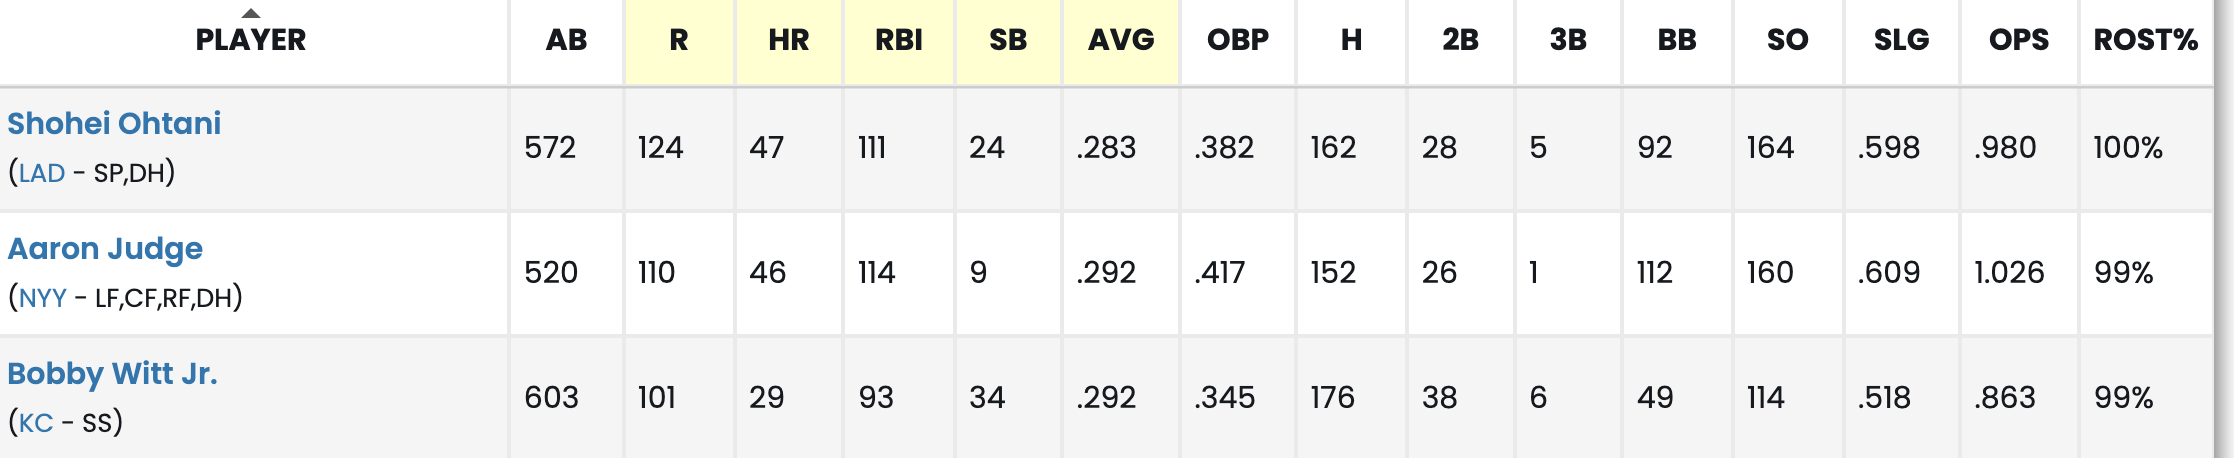
\includegraphics[width=0.9\linewidth]{./image.png}
  \caption{Example of 2026 player projected batting and pitching statistics from FantasyPros \hyperref[ref:fantasypros-proj]{[1]}.}
  \label{fig:projected_data}
\end{figure}

\begin{figure}[H]
  \centering
  
\includegraphics[width=0.8\linewidth]{./image-1.png}
  \caption{Example of player Average Draft Position (ADP) from FantasyPros consensus ADP \hyperref[ref:fantasypros-adp]{[2]}.}
  \label{fig:player_adp}
\end{figure}

Player values are calculated using two distinct standard scoring benchmarks: Yahoo (which focuses on traditional counting stats) \hyperref[ref:yahoo-scoring]{[3]} and FanGraphs (incorporates more advanced player metrics based on linear weights) \hyperref[ref:fangraphs-scoring]{[4]}. The detailed weights for both batters and pitchers are outlined in Table \ref{tab:scoring_weights}:

\begin{table}[H]
\centering
\caption{Scoring weights for Yahoo and FanGraphs/Ottoneu formats \hyperref[ref:yahoo-scoring]{[3]}, \hyperref[ref:fangraphs-scoring]{[4]}.}
\label{tab:scoring_weights}
\small
\begin{tabular}{l c c | l c c}
\toprule
\multicolumn{3}{c|}{\textbf{Batters}} & \multicolumn{3}{c}{\textbf{Pitchers}} \\
\textbf{Metric} & \textbf{Yahoo} & \textbf{FanGraphs} & \textbf{Metric} & \textbf{Yahoo} & \textbf{FanGraphs} \\
\midrule
1B (or H) & 2.6 & 5.6 & IP  & 3.0 & 7.4 \\
2B        & 5.2 & 2.9 & K   & 3.0 & 2.0 \\
3B        & 7.8 & 5.7 & W   & 8.0 & --  \\
HR        & 10.4& 9.4 & SV  & 8.0 & 5.0 \\
R         & 1.9 & --  & ER  & -3.0& --  \\
RBI       & 1.9 & --  & BB  & -1.3& -3.0\\
BB        & 2.6 & 3.0 & H   & -1.3& -2.6\\
SB        & 4.2 & 1.9 & HBP & -1.3& -3.0\\
HBP       & 0 (2.6) & 0 (3.0) & HR  & --  &-12.3\\
AB        & --  &-1.0 & HLD & --  & 4.0 \\
CS        & --  &0 (-2.8) &     &     &     \\
\bottomrule
\end{tabular}
\end{table}

Slight modifications were made to the original projected stats to align with these scoring categories \hyperref[ref:yahoo-scoring]{[3]}, \hyperref[ref:fangraphs-scoring]{[4]}. For example, since Hit By Pitch (HBP) and Caught Stealing (CS) for batters are lacked in the raw stats, we effectively set their scoring weights to zero (original standard weights are shown in parentheses in the table). 

Additionally, across all experiments (both real and synthetic data), the manager's initial draft position is standardized to the middle of the draft order (e.g., the 6th pick in a 12-team league) to maintain a consistent evaluation baseline.

\subsection{Experimental Synthetic Data Generation}

While real data confirms practical viability, a further validation is performed on synthetic data. The generated data is indispensable as it allows us to mathematically isolate specific operational variables (Factors) — such as talent distribution, positional versatility, and market supply — and stress-test the algorithms under controlled extreme conditions. 

The total number of generated players in the environment is defined dynamically based on the league size ($T$), base roster slots ($R = 16$), roster scale multiplier ($S$), and player-demand ratio ($D$): 
\[ N_{\text{players}} = S \times 16 \times T \times D \]

Experimental framework generates synthetic profiles encompassing 4 primary operational factors:

\subsection{Factor A: Points Distribution (\texorpdfstring{$v_i$}{vi})}
We designed three points distributions to simulate different talent pools, clipping all generated values to a realistic range of $[10.0, 800.0]$ according to the FantasyPros projection data collected above \hyperref[ref:fantasypros-proj]{[1]}:
\begin{itemize}[leftmargin=1.5em]
    \item \textbf{Normal (Baseline)}: Values follow a normal distribution $v_i \sim \mathcal{N}(400, 120^2)$. This represents an average draft class where the majority of players are solid, mid-tier contributors.
    \item \textbf{Uniform}: Values are uniformly distributed $v_i \sim \mathcal{U}(10, 800)$. This flattens the talent curve, offering many viable replacement options and minimizing scarcity.
    \item \textbf{High-Low (Star-Heavy)}: We simulate a highly skewed draft class. Only $10\%$ of players are classified as elites, with values drawn from $\mathcal{U}(500, 800)$. The remaining $90\%$ fall into $\mathcal{U}(10, 500)$. In this scenario, missing out on top-tier talent may be severely punished in the objective function.
\end{itemize}

\subsection{Factor B: Position Eligibility Distribution (\texorpdfstring{$E_i$}{Ei})}
We control how versatile the player pool is using four distinct generation logics:
\begin{itemize}[leftmargin=1.5em]
    \item \textbf{Roster-Ratio (Baseline)}: Players are assigned exactly one position, but the probability of generating a specific position aligns precisely with roster demand (e.g., more OF and SP players are generated since there shall be 3 such positioned-players per team).
    \item \textbf{Uniform-by-Type}: A player is randomly designated as a hitter or pitcher, then uniformly assigned a position pattern (including dual-eligibility like \texttt{1B;3B} or \texttt{SP;RP}).
    \item \textbf{Point-Flexible}: The generator ranks all players by points. Players in the top 20\% (elite) have an $80\%$ chance of gaining multi-position eligibility (up to 3 positions). This mimics real life where superstars often possess high versatility.
    \item \textbf{Single-Position}: Every player possesses exactly 1 eligible position. This eliminates all flexibility, representing the ultimate test of scarcity, making early greedy mistakes almost impossible to repair.
\end{itemize}

\subsection{Factor C: Market Conditions and ADP Uncertainty ($\sigma_{\text{adp}}$)}
To generate ADP, we first sort all players by their true projected points in descending order to establish a ``True Rank'', then simulate market noise by adding a Gaussian (Normal) error term:
\[ \text{ADP}_i = \text{TrueRank}_i + \mathcal{N}(0, \sigma_{\text{adp}}^2) \]
\begin{itemize}[leftmargin=1.5em]
    \item $\sigma_{\text{adp}} = 0$ represents a perfectly efficient market where opponents draft strictly by objective value.
    \item Higher $\sigma_{\text{adp}}$ indicates market chaos. Opponents may make unpredictable ``reaches'' or leave bargains on the board. This tests how robust our algorithms are when future availability is uncertain.
\end{itemize}

\subsection{Factor D: Player Demand Ratio ($D$)}
To test the algorithms under varying levels of scarcity, we manipulate the Player Demand Ratio ($D$). The factor controls the supply-and-demand economics of the draft pool by dictating the ratio of ``Available Players'' versus ``Total League Demand''. Let $T$ be the number of teams and $R=16$ be the base roster slots, the total number of generated players is strictly governed by $N_{\text{players}} = R \times T \times D$.
\begin{itemize}[leftmargin=1.5em]
    \item \textbf{$D = 1$ (Tight Market)}: The league will draft almost every available player. One greedy mistake means replacing a starter with absolute zero value.
    \item \textbf{$D = 3$ (Baseline Supply)}: Representing standard draft conditions with a typical buffer of free undrafted agents.
    \item \textbf{$D = 10$ (High Abundance)}: The player pool is a massive ocean of options.
\end{itemize}

\subsection{Scenario Matrix}

We developed 12 distinct scenarios to isolate the impact of each factor. As shown in Table~\ref{tab:scenario_matrix}, \textbf{Scenario S1} serves as the baseline for all comparative analyses. The remaining scenarios follow the factor order introduced above: projected points distribution, position eligibility distribution, market conditions, and player demand ratio. For every scenario, we generate \textbf{10 random instances} to calculate the mean ($\mu$) and standard deviation ($\sigma$) of the performance metrics.

\begin{table}[htbp]
\centering
\caption{Experimental Scenario Matrix for Draft Optimization}
\label{tab:scenario_matrix}
\resizebox{\linewidth}{!}{%
\begin{tabular}{clcccc}
\toprule
\textbf{ID} & \textbf{Main Factor} & \textbf{Demand Ratio ($D$)} & \textbf{Points Distribution ($v_i$)} & \textbf{Position Eligibility ($E_i$)} & \textbf{ADP Uncertainty ($\delta, \sigma$)} \\ \midrule
S1 & \textbf{Baseline} & 3 & Normal & Roster-Ratio & (0, 30) \\ 
S2 & Points: Uniform & 3 & \textbf{Uniform} & Roster-Ratio & (0, 30) \\
S3 & Points: Star-Heavy & 3 & \textbf{High-Low} & Roster-Ratio & (0, 30) \\ \midrule
S4 & Pos: Uniform-by-Type & 3 & Normal & \textbf{Uniform-by-Type} & (0, 30) \\
S5 & Pos: Point-Flexible & 3 & Normal & \textbf{Point-Flexible} & (0, 30) \\
S6 & Pos: Single-Position & 3 & Normal & \textbf{Single-Position} & (0, 30) \\\midrule
S7 & Market: Efficient & 3 & Normal & Roster-Ratio & \textbf{(0, 0)} \\
S8 & Market: Mild Noise & 3 & Normal & Roster-Ratio & \textbf{(0, 60)} \\
\midrule
S9 & Market: Chaotic & 3 & Normal & Roster-Ratio & \textbf{(+5, 30)} \\
S10 & Market: Chaotic & 3 & Normal & Roster-Ratio & \textbf{(+10, 30)} \\ \midrule
S11 & Demand: High & \textbf{1} & Normal & Roster-Ratio & (0, 30) \\
S12 & Demand: Low & \textbf{10} & Normal & Roster-Ratio & (0, 30) \\
\bottomrule
\end{tabular}%
}
\end{table}

\subsection{Stress Testing Design}

To evaluate the absolute computational limits of our algorithms relative to the IP benchmark, we moreover design a separate \textbf{Large-Scale Stress Test} outside of the standard factor matrix. Instead of sweeping isolated market parameters, this test scales the raw problem dimensions: Drastically increasing both the available player pool and the roster constraints. The primary objective is to simulate massive, unconstrained draft databases to observe the breaking point of exact optimization (IP) and to validate the asymptotic time efficiency of the OCG heuristic under massive scale.

\section{Performance Evaluation}

Algorithms are evaluated using two primary metrics across 10 random seeds for each scenario:
\begin{itemize}[leftmargin=1.5em]
    \item \textbf{Optimal Gap Ratio (\%)}: The distance from the IP benchmark, defined as $\frac{Z_{\text{IP}} - Z_{\text{Heuristic}}}{Z_{\text{IP}}} \times 100\%$. A lower value indicates higher accuracy.
    \item \textbf{Improvement (\%)}: The direct gain of OCG over the DG baseline, calculated per seed as $\frac{Z_{\text{OCG}} - Z_{\text{DG}}}{Z_{\text{DG}}} \times 100\%$ and reported as $\mu \pm \sigma$.
\end{itemize}
Unless otherwise noted, all synthetic results are reported as Mean $\pm$ Standard Deviation.

\subsection{Real-Data Validation}

As the first step of validation, we ran the algorithms on the real-world 2026 FantasyPros projections with Yahoo and FanGraphs/Ottoneu scoring rules \hyperref[ref:fantasypros-proj]{[1]}, \hyperref[ref:yahoo-scoring]{[3]}, \hyperref[ref:fangraphs-scoring]{[4]}. As seen in Table \ref{tab:real_data}, OCG successfully trims the point loss caused by naive greedy drafting, confirming its practical viability on real MLB data structures before proceeding to the more comprehensive synthetic validations.

\begin{table}[H]
\centering
\caption{Real-data validation (Gap measured in optimal gap ratio versus IP).}
\label{tab:real_data}
\begin{tabular}{llc}
\toprule
Scoring Method & Method & Optimal Gap Ratio \\
\midrule
Yahoo 2026 & Opportunity Cost Greedy & \textbf{0.50\%} \\
 & Direct Greedy & 3.24\% \\
\midrule
FanGraphs 2026 & Opportunity Cost Greedy & \textbf{1.24\%} \\
 & Direct Greedy & 3.36\% \\
\bottomrule
\end{tabular}
\end{table}

\subsection{Factor A: Points Distribution}

Table \ref{tab:factor_1} summarizes the impact of the talent distribution. Under the \textbf{Baseline (Normal)} distribution, OCG achieves a tight gap of 1.92\%, reducing the error of the DG baseline by more than half. The advantage is most pronounced in \textbf{Star-Heavy} markets (S3), where OCG prevents elite talent from being snatched by opponents, yielding a \textbf{6.10\%} average improvement in total roster value.

\begin{table}[H]
\centering
\caption{Results for Factor A: Points Distribution. (the optimality gap (\%) $\pm$ standard deviation.)}
\label{tab:factor_1}
\begin{tabular}{lccc}
\toprule
Level & DG Gap (\%) & OCG Gap (\%) & Improvement (\%) \\
\midrule
Normal (Baseline) & $4.79\% \pm 1.18\%$ & $\mathbf{1.92\% \pm 0.57\%}$ & $3.02\% \pm 1.34\%$ \\
Uniform & $3.24\% \pm 0.77\%$ & $\mathbf{1.44\% \pm 0.59\%}$ & $1.87\% \pm 0.65\%$ \\
High-Low (Star-Heavy) & $8.39\% \pm 2.40\%$ & $\mathbf{2.87\% \pm 1.32\%}$ & $\mathbf{6.10\% \pm 3.46\%}$ \\
\bottomrule
\end{tabular}
\end{table}

\subsection{Factor B: Position Eligibility Distribution}

Table \ref{tab:factor_2} illustrates performance across different positional flexibility environments. Compared to the \textbf{Baseline (Roster-Ratio)}, \textit{point-flexible} is the most forgiving environment (gap drops to 1.34\%) because top players can seamlessly plug holes in the roster. Conversely, \textit{single-position} creates a rigid, unforgiving draft. Even when mistakes are impossible to patch with utility players, OCG dominates Direct Greedy (0.94\% vs 5.11\%), proving that looking one pick ahead prevents catastrophic positional deficits later in the draft.

\begin{table}[H]
\centering
\caption{Results for Factor B: Position Eligibility Distribution.}
\label{tab:factor_2}
\begin{tabular}{lccc}
\toprule
Level & DG Gap (\%) & OCG Gap (\%) & Improvement (\%) \\
\midrule
Roster-Ratio (Baseline) & $4.79\% \pm 1.18\%$ & $\mathbf{1.92\% \pm 0.57\%}$ & $3.02\% \pm 1.34\%$ \\
Uniform-by-Type & $4.89\% \pm 0.62\%$ & $\mathbf{1.07\% \pm 0.43\%}$ & $4.02\% \pm 0.82\%$ \\
Point-Flexible & $5.36\% \pm 1.66\%$ & $\mathbf{1.34\% \pm 0.68\%}$ & $4.27\% \pm 1.83\%$ \\
Single-Position & $5.11\% \pm 1.48\%$ & $\mathbf{0.94\% \pm 0.65\%}$ & $\mathbf{4.42\% \pm 1.95\%}$ \\
\bottomrule
\end{tabular}
\end{table}

\subsection{Factor C: Market Conditions and ADP Uncertainty}

Table \ref{tab:factor_3} demonstrates performance under chaotic draft markets. We split the analysis into two sweeps: varying market noise ($\sigma_{\text{adp}}$) and varying availability tolerance ($\delta$).

When the market is perfectly efficient ($\sigma_{\text{adp}}=0$), predicting opponent behavior is trivial, and both algorithms perform exceptionally well. As noise increases to $\sigma_{\text{adp}}=60$, the draft becomes unpredictable. Direct Greedy struggles significantly (gap over $5\%$), whereas OCG remains highly robust ($2.43\%$). Similarly, whether the availability tolerance ($\delta$) is incredibly strict ($-10$) or highly permissive ($10$), OCG consistently keeps the gap under $2\%$. Because OCG bases its priority on the \textit{relative difference} (Opportunity Cost) rather than absolute values, it inherently hedges against market volatility.

\begin{table}[H]
\centering
\caption{Factor C: Market Conditions and ADP Uncertainty results. The first sweep tests market noise ($\sigma_{\text{adp}}$) with fixed $\delta=0$. The second tests nonnegative tolerance ($\delta$) with fixed $\sigma_{\text{adp}}=30$. Values represent the optimality gap (\%) $\pm$ standard deviation.}
\label{tab:factor_3}
\begin{tabular}{llccc}
\toprule
Sweep & Level & DG Gap (\%) & OCG Gap (\%) & Improvement (\%) \\
\midrule
\textbf{Noise} & $\sigma_{\text{adp}}=0$ (Efficient) & $1.47\% \pm 0.48\%$ & $\mathbf{0.48\% \pm 0.23\%}$ & $1.00\% \pm 0.50\%$ \\
 & $\sigma_{\text{adp}}=30$ (Moderate) & $4.79\% \pm 1.18\%$ & $\mathbf{1.92\% \pm 0.57\%}$ & $3.02\% \pm 1.34\%$ \\
 & $\sigma_{\text{adp}}=60$ (Chaotic) & $5.56\% \pm 1.58\%$ & $\mathbf{2.43\% \pm 1.55\%}$ & $\mathbf{3.33\% \pm 1.43\%}$ \\
\midrule
\textbf{Tolerance} & $\delta=0$ (Baseline) & $4.79\% \pm 1.18\%$ & $\mathbf{1.92\% \pm 0.57\%}$ & $3.02\% \pm 1.34\%$ \\
 & $\delta=+5$ & $5.54\% \pm 1.57\%$ & $\mathbf{1.64\% \pm 0.75\%}$ & $\mathbf{4.16\% \pm 1.50\%}$ \\
 & $\delta=+10$ (Permissive) & $5.42\% \pm 1.21\%$ & $\mathbf{1.72\% \pm 0.95\%}$ & $3.92\% \pm 1.03\%$ \\
\bottomrule
\end{tabular}
\end{table}

\subsection{Factor D: Player Demand Ratio}

Table \ref{tab:factor_4} highlights scaling under tight vs. loose supply (Player Demand Ratio $D$). When supply is brutally tight ($D=1$, meaning almost every player must be drafted), Direct Greedy collapses (8.81\% gap) as it blindly paints itself into a corner. OCG, aware of the impending scarcity, navigates the tight market with only a 2.64\% gap. In a high-abundance scenario ($D=10$), OCG drops the error rate to a mere $1.16\%$.

\begin{table}[H]
\centering
\caption{Factor D: Player Demand Ratio results (Fixed Roster Scale = 1). Values represent the optimality gap (\%) $\pm$ standard deviation.}
\label{tab:factor_4}
\begin{tabular}{lccc}
\toprule
Level & DG Gap (\%) & OCG Gap (\%) & Improvement (\%) \\
\midrule
D = 3 (Baseline) & $4.79\% \pm 1.18\%$ & $\mathbf{1.92\% \pm 0.57\%}$ & $3.02\% \pm 1.34\%$ \\
D = 1 (Demand: High) & $8.81\% \pm 2.19\%$ & $\mathbf{2.64\% \pm 1.23\%}$ & $\mathbf{6.82\% \pm 3.13\%}$ \\
D = 10 (High Abundance) & $3.29\% \pm 0.85\%$ & $\mathbf{1.16\% \pm 0.51\%}$ & $2.20\% \pm 0.83\%$ \\
\bottomrule
\end{tabular}
\end{table}

\subsection{Large-Scale Stress Testing}

This section presents the most critical argument for our front office pitch: \textbf{Scalability}. While the IP finds perfect rosters in smaller instances, what happens when the scouting department dumps a universe of hundreds of thousands of eligible players into the database?

Table \ref{tab:stress_time} showcases the \textbf{Large-Scale Stress Test}. To understand the complexity of the IP, we approximate its search space by the variable count. For $n$ available players, $p$ roster positions, and a roster size of $r$, the approximate number of decision variables is:
\[ \text{Approx. Variables} = n \times (1 + p + r) \]
This formula encompasses the player-selection variables ($y_i$), player-position assignment variables ($x_{ip}$), and player-round availability variables ($z_{ik}$). As we scale the roster size to 256 and the player pool to 184,320, the approximate variable count reaches nearly 50 million.

The Branch-and-Bound tree of the IP explores an exponentially growing space. As a result, the IP runtime explodes from 4 seconds to 276 seconds, and eventually hits our predefined 30-minute (1800 seconds) solver time limit for the largest target, triggering a \texttt{TIMEOUT\_ERROR}. In stark contrast, confirming our $O(n \log n)$ complexity analysis, \textbf{Opportunity Cost Greedy processes the massive 50-million variable equivalent environment in just 23.286 seconds}.


\begin{table}[H]
\centering
\small
\caption{Stress Test: Execution Times for DG, OCG, and IP.}
\label{tab:stress_time}
\resizebox{\linewidth}{!}{%
% We split the time column into 3 sub-columns aligned on the slashes
\begin{tabular}{lrrr r @{ / } r @{ / } r rr}
\toprule
Level & Players & Teams & Picks & \multicolumn{3}{c}{DG / OCG / IP Time(s)} & DG Gap (\%) & OCG Gap (\%) \\
\midrule
Small  & 5,760 & 12 & 48 & 0.790 & 0.852 & 4.235 & 2.430\% & \textbf{1.098\%} \\
Medium & 9,600 & 15 & 64 & 0.951 & 1.144 & 12.230 & 1.771\% & \textbf{0.646\%} \\
Large  & 21,600 & 15 & 96 & 1.981 & 2.344 & 54.267 & 0.940\% & \textbf{0.407\%} \\
XLarge & 64,000 & 20 & 160 & 6.172 & 10.360 & 276.895 & 0.270\% & \textbf{0.137\%} \\
Target & 184,320 & 24 & 256 & 17.760 & 23.286 & \textbf{TIMEOUT} &   -- & -- \\
\bottomrule
\end{tabular}
}
\end{table}

\begin{figure}[H]
  \centering
  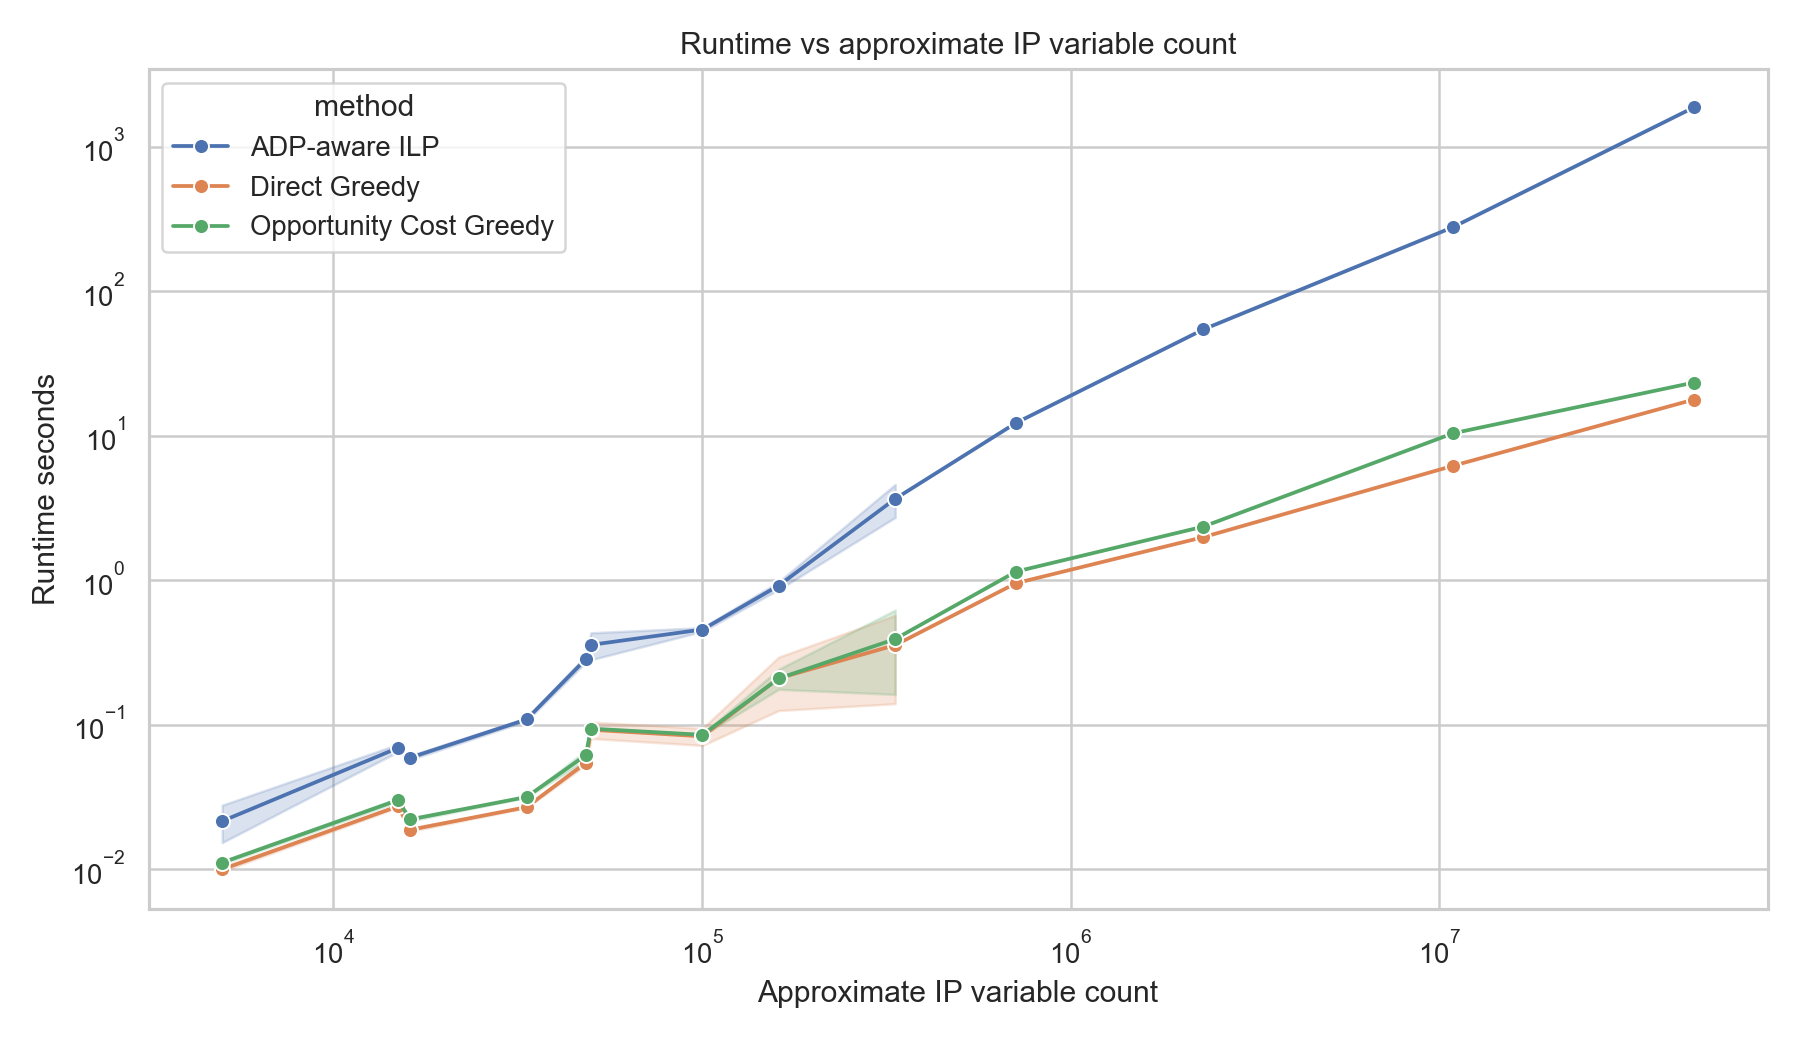
\includegraphics[width=0.75\linewidth]{./runtime_by_variable_count.png}
  \caption{Runtime comparison for Stress Tests. IP scales exponentially while heuristics scale linearly.}
\end{figure}

\subsection{Strategic Insights and Competitive Edge}

After evaluating the algorithm across 12 distinct scenarios, we identify the conditions where the \textbf{Opportunity Cost Greedy (OCG)} algorithm provides the most significant strategic advantage. Table \ref{tab:highlights} highlights the top-performing scenarios based on the improvement over the baseline.

\begin{table}[H]
\centering
\caption{Key Strategic Scenarios: Maximum Improvement of OCG over DG.}
\label{tab:highlights}
\resizebox{\linewidth}{!}{%
\begin{tabular}{lllc}
\toprule
\textbf{Factor} & \textbf{Scenario ID} & \textbf{Environment Condition} & \textbf{Improvement (\%)} \\
\midrule
\textbf{Points Distribution (Factor A)} & S3 & Points: Star-Heavy & \textbf{+6.10\%} \\
\textbf{Position Eligibility (Factor B)} & S6 & Pos: Single-Position & \textbf{+4.42\%} \\
\textbf{Market Conditions (Factor C)} & S9 & Market: Chaotic ($\delta=+5$) & \textbf{+4.16\%} \\
\textbf{Player Demand Ratio (Factor D)} & S11 & Demand: High ($D=1$) & \textbf{+6.82\%} \\
\bottomrule
\end{tabular}
}
\end{table}

\noindent \textbf{Analysis of the Competitive Edge:}
The highlighted scenarios reveal where cost-of-delay reasoning matters most. In star-heavy drafts (S3), OCG secures elite assets before the value cliff occurs. Under single-position eligibility (S6), it prevents early positional mistakes that cannot be repaired later. In chaotic markets (S9), the delay-cost heuristic remains robust to uncertain opponent behavior. Finally, in high-demand environments (S11), OCG avoids DG's ``positional blindness'' and prevents late-draft roster collapses.


\subsection{Competitive Market Simulation}

To evaluate OCG in a multi-agent environment, we implemented a 12-team draft simulation. Unlike the previous IP-benchmark experiments, this test measures how one OCG-managed team performs while competing directly against 11 DG-managed teams for the same player pool.

\textbf{Methodology:}
Using real-world 2026 FantasyPros projections, FantasyPros ADP, and Yahoo/FanGraphs scoring rules, we ran 12 separate snake drafts and shifted the OCG team's starting position from the 1st pick to the 12th pick \hyperref[ref:fantasypros-proj]{[1]}, \hyperref[ref:fantasypros-adp]{[2]}, \hyperref[ref:yahoo-scoring]{[3]}, \hyperref[ref:fangraphs-scoring]{[4]}. All teams followed the same roster requirements and market availability rules.

\textbf{Results and Analysis:}
Figure \ref{fig:competitive_simulation} compares the OCG team's objective and rank against DG opponents across all draft positions. OCG achieves first place across all Yahoo positions and first or second place across all FanGraphs positions. This suggests that cost-of-delay reasoning remains robust even when multiple agents compete for the same scarce resources.

\begin{figure}[H]
    \centering
    \vspace{-0.6em}
    \begin{minipage}[t]{0.42\linewidth}
        \centering
        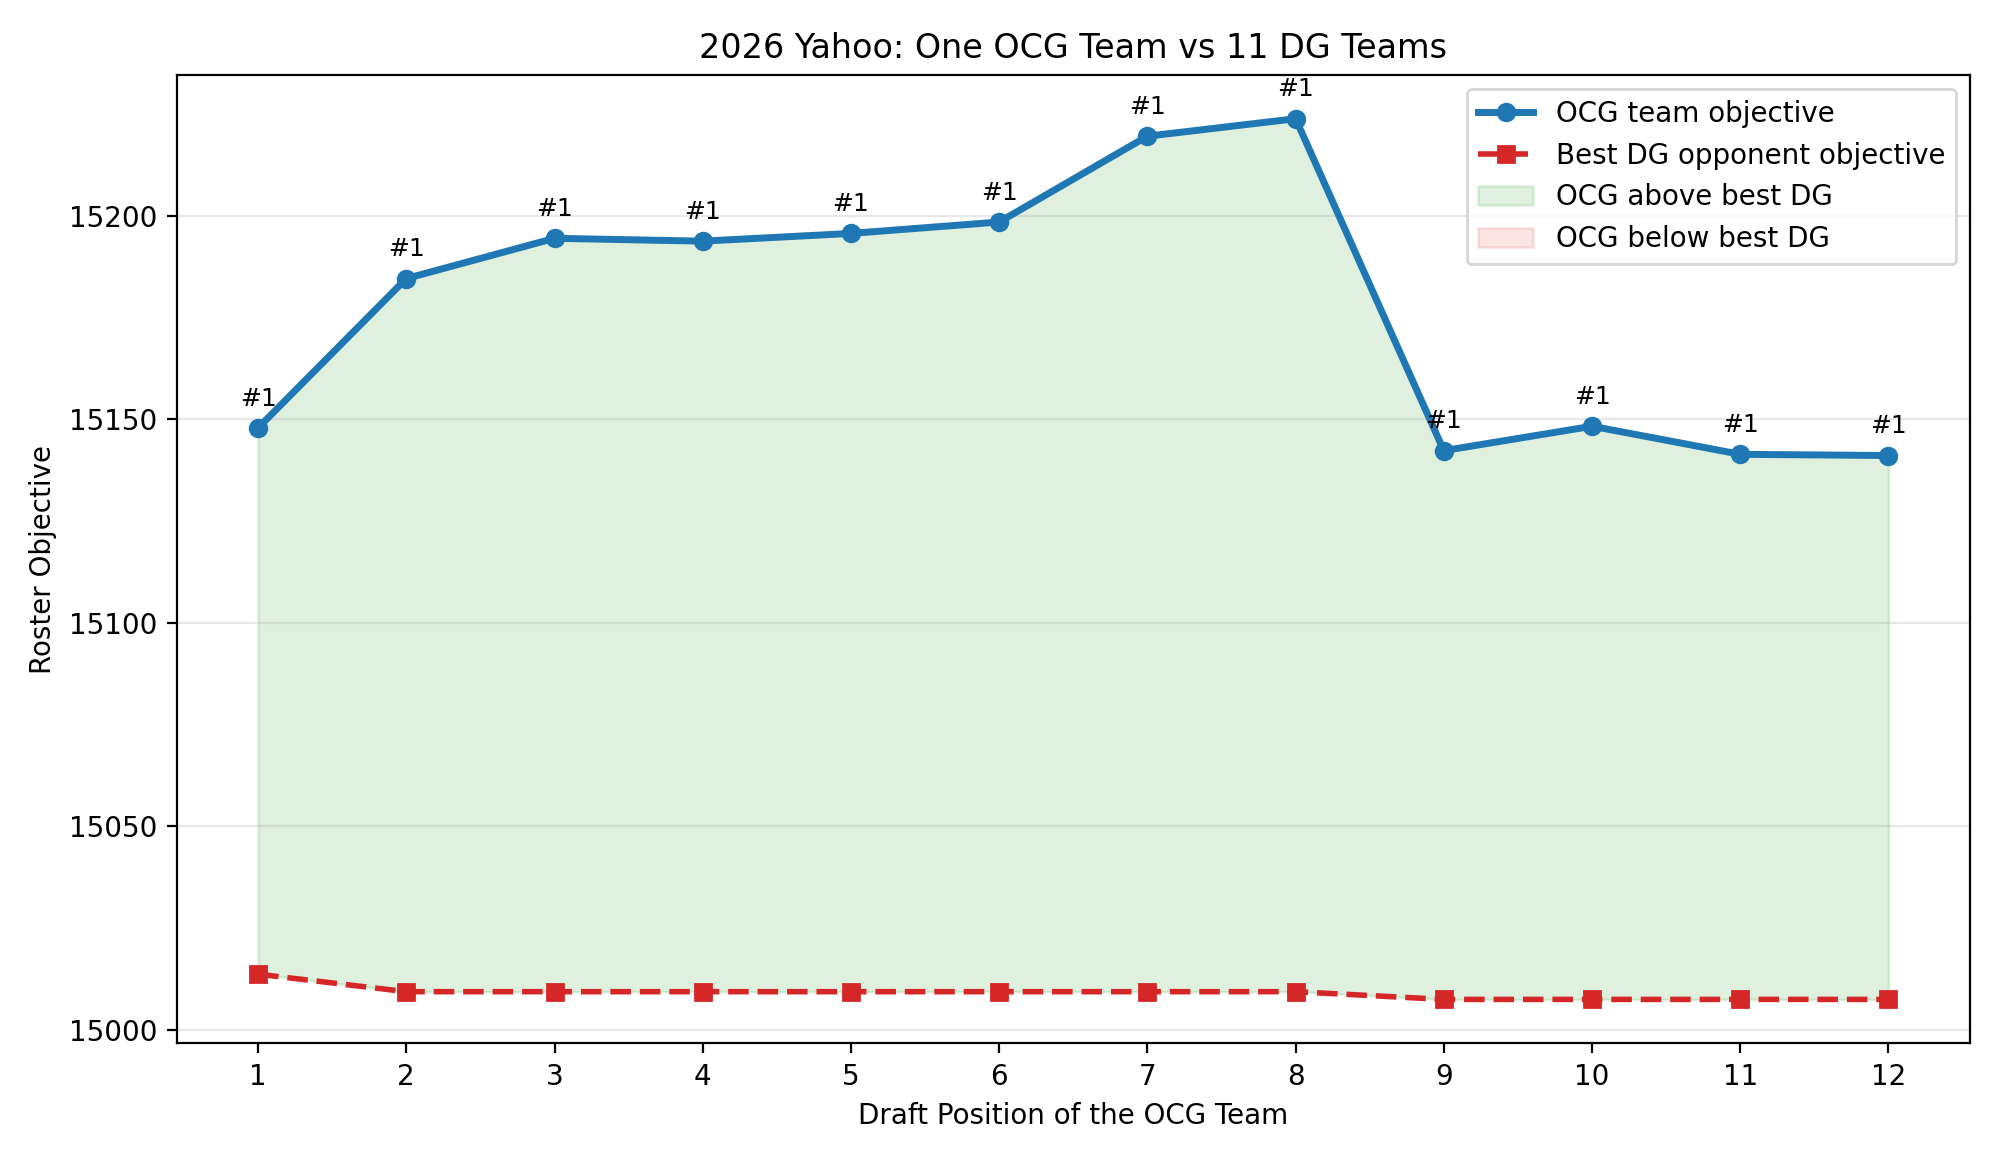
\includegraphics[width=\linewidth]{./ocg_vs_dg_yahoo_by_draft_position.png}
    \end{minipage}
    \hfill
    \begin{minipage}[t]{0.42\linewidth}
        \centering
        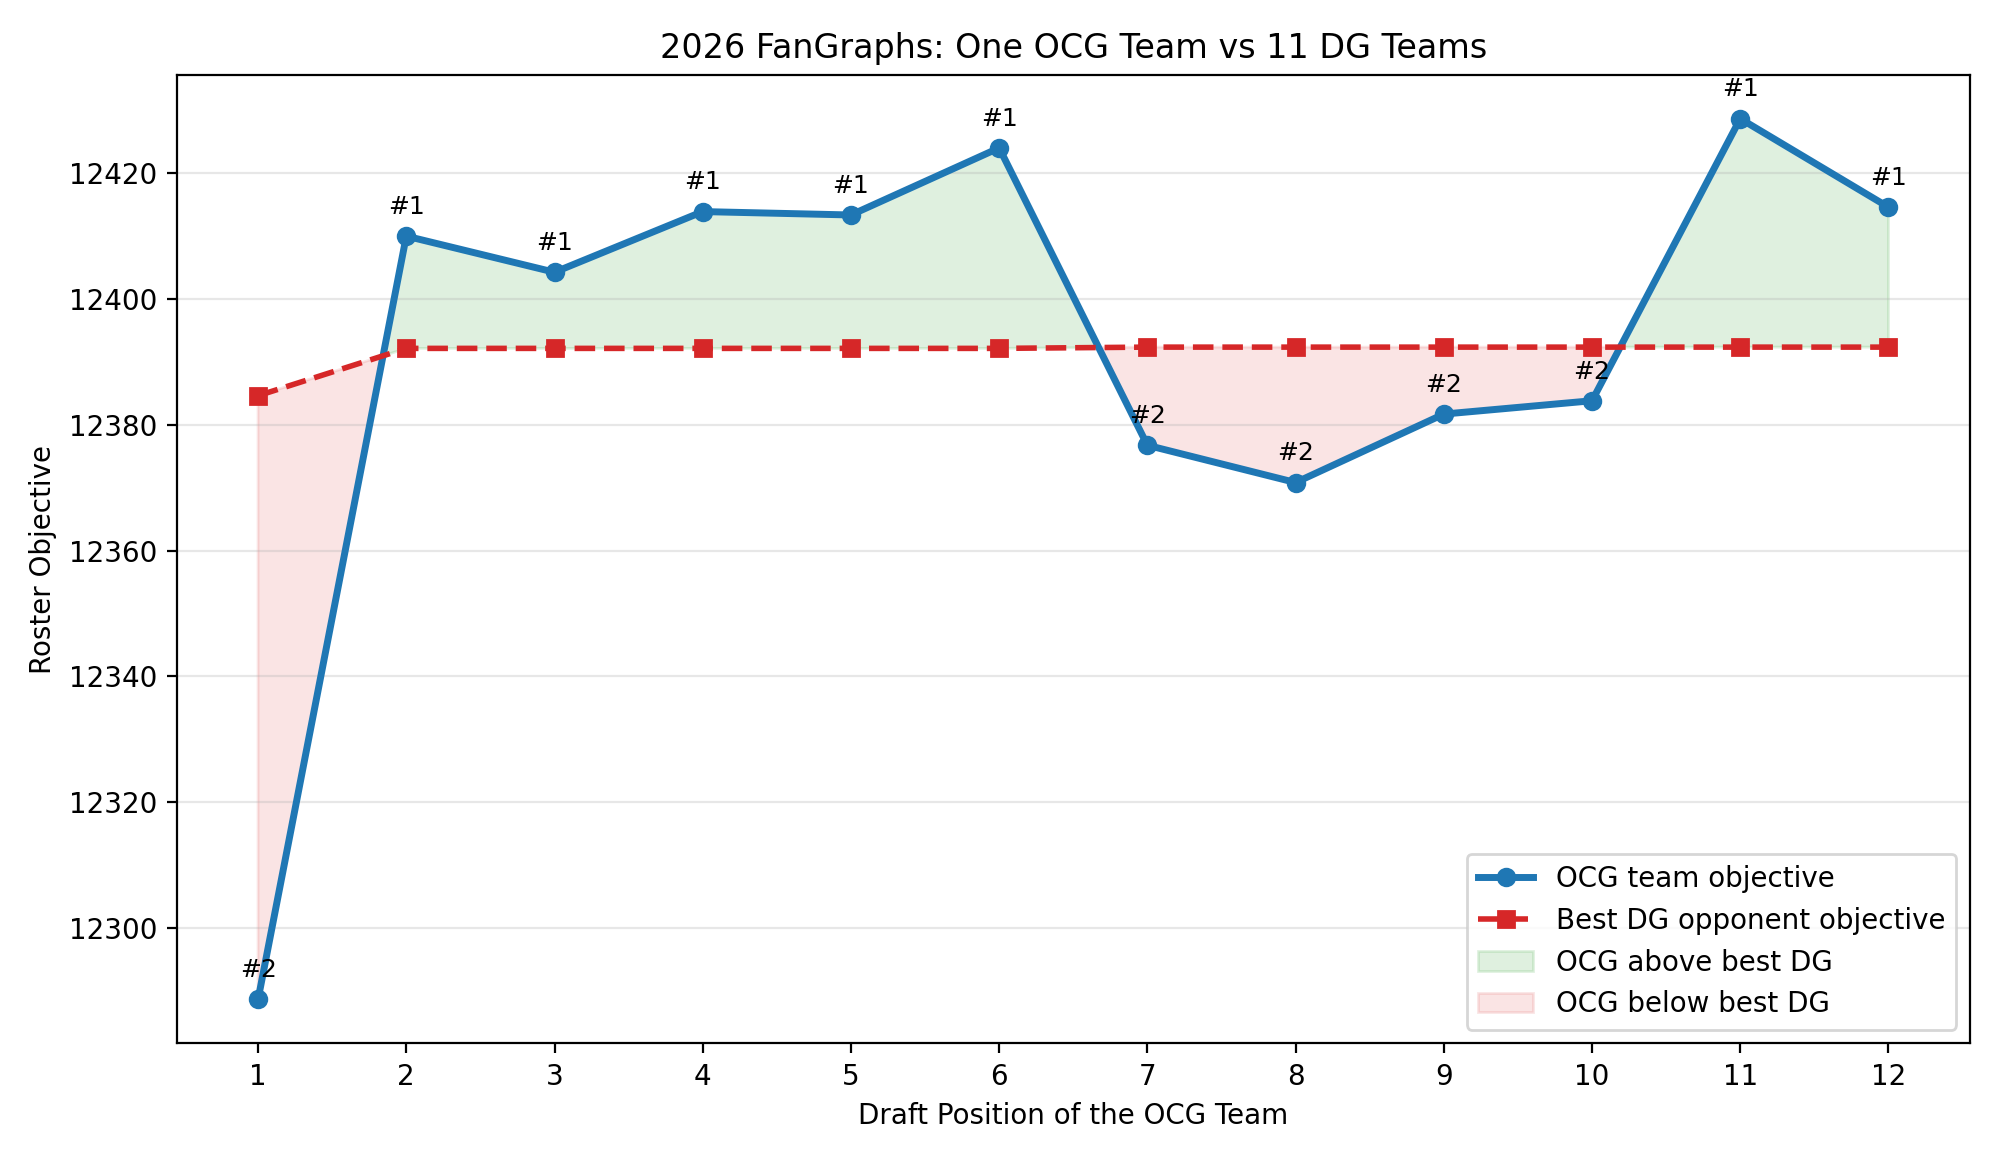
\includegraphics[width=\linewidth]{./ocg_vs_dg_fangraph_by_draft_position.png}
    \end{minipage}
    \vspace{-0.6em}
    \caption{Competitive simulation: one OCG team vs. 11 DG teams across all draft positions. Left: Yahoo; right: FanGraphs. OCG ranks first for Yahoo and either first or second for FanGraphs.}
    \label{fig:competitive_simulation}
    \vspace{-0.8em}
\end{figure}


\section{Conclusions and Strategic Outlook}

The results of this project demonstrate that roster construction in competitive markets is a complex sequential decision problem that can be effectively addressed through systematic optimization logic. By utilizing Fantasy Baseball as a data-rich testbed, we have evaluated the balance between theoretical Integer Programming and real-time decision support. Based on our evaluations, we draw the following conclusions:

\begin{enumerate}[leftmargin=1.5em, itemsep=2pt, topsep=4pt]
    \item \textbf{Bridging Optimality and Scalability:} While Integer Programming (IP) provides a rigorous benchmark, its exponential worst-case complexity makes it impractical for large-scale live environments. Our proposed \emph{Opportunity Cost Greedy (OCG)} algorithm reduces the decision process to near-linear operations ($O(n \log n + r \cdot p)$). In standard league sizes, OCG maintains sub-second latency, and in extreme stress tests, it processes approximately 50 million decision variables in under 25 seconds while remaining within a roughly 1--2\% gap of the IP benchmark.
    \item \textbf{Resilience against ``Value Cliffs'':} The strategic core of OCG is its ability to quantify the \textbf{cost-of-delay}. In environments characterized by star-heavy distributions or high demand, myopic strategies often ignore the impending depletion of specific positions. OCG identifies these ``Value Cliff'' thresholds by looking ahead to the next pick, prioritizing scarce assets whose utility is expected to decline sharply. This robust look-ahead decision policy results in significant utility gains, particularly in scenarios with limited positional flexibility.
    \item \textbf{Robustness in Competitive Ecosystems:} Multi-agent simulations indicate that OCG remains effective when competing against multiple DG agents for a shared player pool. In 2026 real-data simulations, the OCG agent consistently ranked first across all draft positions in the Yahoo setting, and remained in either first or second place throughout the draft order in the FanGraphs setting. This suggests that delay-cost logic translates into a tangible strategic advantage in realistic, multi-agent environments.
\end{enumerate}

\textbf{Future Extensions:} 
Future research could transition this deterministic framework toward \textbf{Stochastic Opponent Modeling}. By incorporating probability distributions of opponent behavior instead of fixed ADP thresholds, the model could calculate expected opportunity costs more accurately. 

Furthermore, integrating \textbf{Risk-Aware Utility} via Monte Carlo simulations would account for player injury risks and performance volatility. From a broader perspective, the underlying logic is highly generalizable beyond sports; it provides a foundational framework for any \textbf{sequential resource procurement} or \textbf{talent acquisition} scenario where multiple agents must secure scarce, heterogeneous assets under real-time pressure and competitive depletion.

\section*{References}

{\small
\begin{sloppypar}
\begin{enumerate}[label={[\arabic*]}, leftmargin=2em, itemsep=2pt]
    \item \label{ref:fantasypros-proj}\textbf{FantasyPros.} \textit{2026 MLB Player Projected Statistics (Batting/Pitching).} \url{https://www.fantasypros.com/mlb/projections/}
    \item \label{ref:fantasypros-adp}\textbf{FantasyPros.} \textit{2026 Fantasy Baseball Average Draft Position (ADP) Consensus.} \url{https://www.fantasypros.com/mlb/adp/overall.php}
    \item \label{ref:yahoo-scoring}\textbf{Yahoo Sports.} \textit{Default League Settings and Head-to-Head Points Scoring System.} \url{https://help.yahoo.com/kb/default-league-settings-fantasy-baseball-sln6785.html}
    \item \label{ref:fangraphs-scoring}\textbf{FanGraphs / Justin Merry.} \textit{Ottoneu Scoring and Linear Weights for Sabermetric Evaluation.} \url{https://ottoneu.fangraphs.com/support}
\end{enumerate}
\end{sloppypar}
}

\end{document}
